\subsection{Оптическая толщина. Закон Бугера}
\begin{wrapfigure}[10]{c}{0.4\tw}
	\centering
	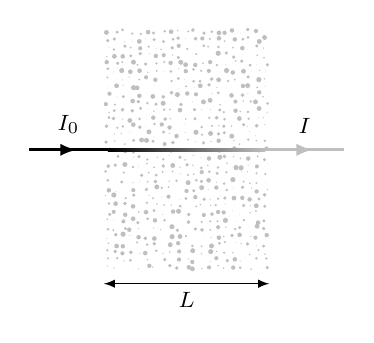
\begin{tikzpicture}
		\footnotesize
		
		\foreach \x in {-1, -.9, ..., 1.01} {
		\foreach \y in {-1.5, -1.4, ..., 1.51} {
		\pgfmathsetmacro\radius{(rand+1)/60};
		\fill [lightgray] (\x + rand*.03, \y + rand*.03)  circle(\radius);
		};
		};
		
		\draw [line width=1pt](-2, 0) -- (-1, 0);
		\draw [line width=1pt, -latex](-2, 0) -- (-1.4, 0);
		\fill[left color=black, right color=lightgray] (-1, -.5pt) rectangle (1, .5pt);
		\draw [line width=1pt, lightgray](1, 0) -- (2, 0);
		\draw [line width=1pt, lightgray, -latex](1, 0) -- (1.6, 0);
		
		\draw (-1.5, .1) node[anchor=south] {$I_0$};
		\draw (1.5, .1) node[anchor=south] {$I$};
		
		\draw [latex-latex] (-1.05, -1.7) -- (1.05, -1.7);
		\draw (0, -1.7) node[anchor=north] {$L$};
	\end{tikzpicture}
	\caption{}
	\label{}
\end{wrapfigure}
Рассмотрим прохождение электромагнитного излучения с интенсивностью $I_0$ через слой толщины $L$ непрозрачных частиц со средней концентрацией $n$ и сечением поглощения $\sigma$. Ясно, что интенсивность выходящего из слоя пыли излучения будет меньше начальной. Выясним, по какому закону падает интенсивность излучения в таком случае.

Для этого рассмотрим тонкий слой толщины $dx$ из всего слоя частиц. Пусть на входе в этот тонкий слой излучение имеет интенсивность $I$, а на выходе из слоя~--- $I - dI$. Часть излучения прошла сквозь тонкий слой, а часть поглотилась пылинками, общая площадь которых равна произведению их количества в этом слое на среднюю площадь поглощения. Здесь можно считать, что перекрытия частиц друг другом не происходит, так как рассматриваемый слой достаточно тонкий. Количество частиц  $dN$ в тонком слое зависит только от их концентрации и площади всего слоя, таким образом:
\begin{equation*}
	N = n S \, dx.
\end{equation*}
Тогда можно составить уравнение на изменение интенсивности излучения тонким слоем:
\begin{equation*}
	-\frac{dI}{I} = \frac{N\sigma}{S} = n\sigma \, dx.
\end{equation*}
Проинтегрируем левую и правую часть полученного уравнения:
\begin{gather*}
	-\int\limits_{I_0}^{I} \frac{dI}{I} = \int\limits_{0}^{L} n \sigma \, dx,\\
	-\ln I + \ln I_0 = n\sigma L,\\[.5pc]
	%	e^{-\ln I_0} \cdot e^{\ln I} = e^{n \sigma L},
	I = I_0 e^{-n\sigma L}. \tag{\theequation}
\end{gather*}

\term{Оптическая толщина}~--- безразмерная величина, характеризующая степень непрозрачности среды для проходящего сквозь неё излучения. В общем случае, конечно, концентрация частиц и их площадь сечения взаимодействия могут меняться от координаты, поэтому оптическая толщина определяется как
\begin{equation}
	\tau = \int n(x) \sigma(x)\,dx.
\end{equation}
Для случая постоянных $n$ и $\sigma$, как было получено выше, $\tau = n \sigma L$.

Связь интенсивности $I_0$ на входе с интенсивностью $I$ на выходе называется \term{Законом Бугера} и записывается в виде
\begin{equation}
	I = I_0 e^{-\tau}.
\end{equation}

